\documentclass{article}
	\usepackage[utf8]{inputenc}
	\usepackage{float}
	\usepackage{pdfpages}
	\usepackage[T1]{fontenc}
	\usepackage{float}
	\usepackage{booktabs}
	\usepackage{multirow}
	\usepackage{ragged2e}
	\usepackage{makecell}
	\renewcommand{\theadfont}{\small\bfseries}
	\usepackage{tabularx}
	\usepackage[autolanguage, np]{numprint}
	\newcolumntype{Z}{ >{\centering\arraybackslash}X }
	\usepackage{makecell}
	\usepackage{url}
	\usepackage{siunitx}
	\usepackage{caption}
	\usepackage[framemethod=TikZ]{mdframed}
	\usepackage{tikz, tabularx}
	\usepackage[T1]{fontenc}
	\usepackage{charter}

%%% Document Properties and Packages used 9/20
\usepackage{amsmath}        % math formulas
\usepackage{bm}             % bold math symbols
\usepackage{multicol}       % multiple columns
\usepackage[super]{nth}     % 1st, 2nd, 3rd, 4th
\usepackage{enumitem}       % ordered list (a), (b), (c)
\usepackage{graphicx}		% insert images
\graphicspath{ {./images/} }
\usepackage{geometry}
\geometry{letterpaper, margin=1in, top=0.5in} % small margins
\usepackage{biblatex}		% bibliography
\addbibresource{HW1N1.bib}
%%%%%%%%%%%%%%%%%%%%%%%%%%%%%%%%%%%%%%%%%%%%%%%%%%%%%%%%%%%%%%%%%%%%%%%%%%%%%%%
%%% Code Listing 
\usepackage{listings}
\usepackage{xcolor}

\definecolor{codegreen}{rgb}{0,0.6,0}
\definecolor{codegray}{rgb}{0.5,0.5,0.5}
\definecolor{codepurple}{rgb}{0.58,0,0.82}
\definecolor{backcolour}{rgb}{0.95,0.95,0.92}

\lstdefinestyle{mystyle}{
	backgroundcolor=\color{backcolour},   
	commentstyle=\color{codegreen},
	keywordstyle=\color{magenta},
	numberstyle=\tiny\color{codegray},
	stringstyle=\color{codepurple},
	basicstyle=\ttfamily\footnotesize,
	breakatwhitespace=false,         
	breaklines=true,                 
	captionpos=b,                    
	keepspaces=true,                 
	numbers=left,                    
	numbersep=5pt,                  
	showspaces=false,                
	showstringspaces=false,
	showtabs=false,                  
	tabsize=2
}
\lstset{style=mystyle}
%%%%%%%%%%%%%%%%%%%%%%%%%%%%%%%%%%%%%%%%%%%%%%%%%%%%%%%%%%%%%%%%%%%%%%%%%%%%%%%
\begin{document}
	
	\noindent\textbf{Justine John "JJ" A. Serdoncillo}
	\hfill \textbf{AEM 5253: Computational Fluid Dynamics} \\ \hfill \textbf{December 10, 2022}
	
	\begin{center}
		\Large{\textbf{Homework 3}}    
	\end{center}
	
	\section*{Number 1 a)}
		Below is the plot for the diffusion equation using Runge-Kutta 4th Order Method. The time step used is 0.0125s as shown in the written work. It can be seen that the numerical solution at t=4s matches exactly on top of the analytical solution.

		\begin{figure}[H]
			\centering
			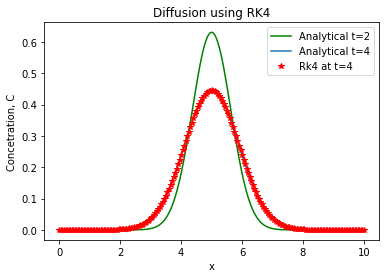
\includegraphics[width=0.6\textwidth]{images/rk4.png}
			\caption{\label{} 1a) Diffusion Equation using Runge-Kutta 4 }
		\end{figure}

	\section*{Number 1 b)}
		Below is the plot for the diffusion equation using Crank-Nicolson method. Upon experimenting with various time steps. It can be seen that it is stable even for high values of dt. The time step used below is t=1s which is the highest possible value that would make sense in this case. It can be seen that the numerical solution at t=4s still matches exactly on top of the analytical solution.
		
		\begin{figure}[H]
			\centering
			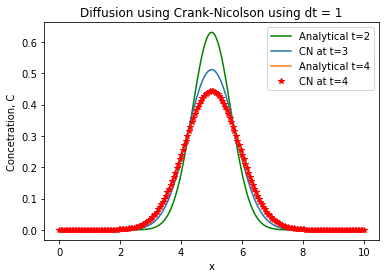
\includegraphics[width=0.6\textwidth]{images/cn.png}
			\caption{\label{} 1b) Diffusion Equation using Crank-Nicolson }
		\end{figure}

	\section*{Number 2)}
		Given the boundary conditions of the rectangular copper plate and the Laplace's equation, the analytical solution of the steady state was given and can be shown by the plot below.
		
		\begin{figure}[H]
			\centering
			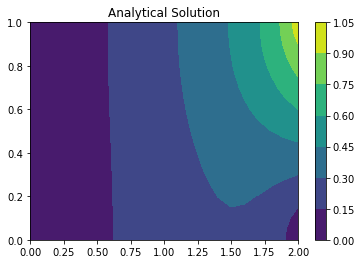
\includegraphics[width=0.6\textwidth]{images/anal.png}
			\caption{\label{} 2) Analytical Solution of the Laplace Equation }
		\end{figure}
	
		For this problem, this will be solved iteratively by using the given equation for the residual and prescribing a tolerance of $ 10^{-6}$
	
	\section*{Number 2 a)}
		The figure below shows the equation solved using Jacobi. The number of iterations can be seen at the summary at the end. 
		
		\begin{figure}[H]
			\centering
			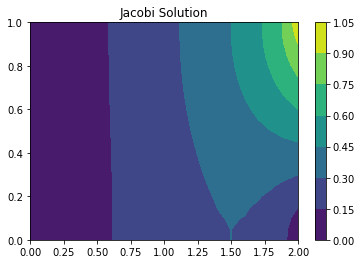
\includegraphics[width=0.6\textwidth]{images/jaco.png}
			\caption{\label{} 2a) Laplace Equation using Jacobi }
		\end{figure}
	
		\begin{figure}[H]
			\centering
			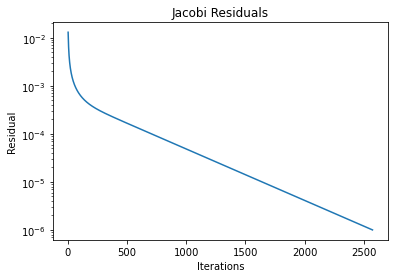
\includegraphics[width=0.6\textwidth]{images/jacores.png}
			\caption{\label{} 2a) Residuals from Laplace Equation using Jacobi }
		\end{figure}
	
	\section*{Number 2 b)}
		The figure below shows the equation solved using Gauss-Seidel. It can be seen that it converges earlier than than the Jacobi solution. Using this method can have a bias when doing the i or j index first but when run both cases, did not pose any difference to the number of iterations.
		
		\begin{figure}[H]
			\centering
			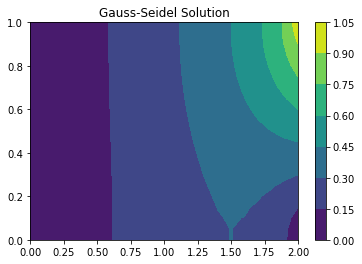
\includegraphics[width=0.6\textwidth]{images/gase.png}
			\caption{\label{} 2b) Laplace Equation using Gauss-Seidel }
		\end{figure}
		
		\begin{figure}[H]
			\centering
			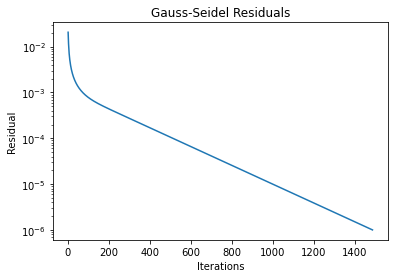
\includegraphics[width=0.6\textwidth]{images/gaseres.png}
			\caption{\label{} 2b) Residuals from Laplace Equation using Gauss-Seidel }
		\end{figure}
	
	\section*{Number 2 c)}
		The Successive-Over Relaxation (SOR) method was used across multiple values of w. The effect of w on iterations can be seen below. It can be seen that most of the iterations were higher than 2000 which was used as a ceiling. This shows that when using the wrong w, it can be more expensive to use.
		
		\begin{figure}[H]
			\centering
			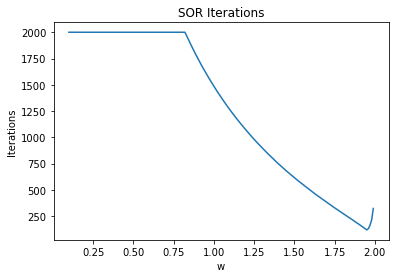
\includegraphics[width=0.6\textwidth]{images/sorite.png}
			\caption{\label{} 2c) Effect of w on iterations using SOR }
		\end{figure}
		
		Using w=1.95 produced the lowest number of iterations and is used to produce the plot below.
		
		\begin{figure}[H]
			\centering
			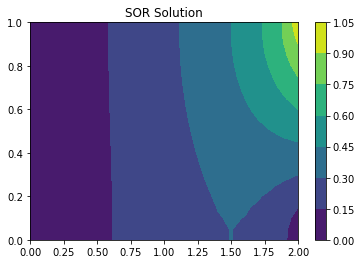
\includegraphics[width=0.6\textwidth]{images/sor.png}
			\caption{\label{} 2c) Laplace Equation using SOR }
		\end{figure}
		
		\begin{figure}[H]
			\centering
			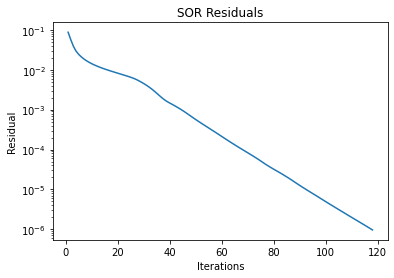
\includegraphics[width=0.6\textwidth]{images/sorres.png}
			\caption{\label{} 2c) Residuals from Laplace Equation using SOR }
		\end{figure}
		 
		
		The table below shows the number of iterations to convergence using the different methods.
		\begin{table}[h!]
			\centering
			\small
			\begin{tabular}{| *{4}{c|}}
				\hline
				\thead{} & \thead{Jacobi} & \thead{Gauss-Seidel} & \thead{SOR}\\
				\hline
				Iterations & 2574 & 1486 & 118 \\
				\hline
				Final Residual & 9.978e-7 & 9.976e-7 & 9.643 \\
				\hline
			\end{tabular}
			\caption{Validation Accuracy vs. Type of Activation Function with no Softmax}
		\end{table}	
		
		
		It can be seen from above that although all of the methods gave substantial results compared to the analytical solution, the number of iterations is drastically different. Gauss-Seidel is better than Jacobi. Using SOR drastically decreases the iterations given that the right value of w is used. If not, then it will be more computationally expensive to do so. 
		
		\section*{Appendix)}
			\subsection*{ Python Code for 1 }
			\lstinputlisting[language=Python]{HW3N1v2.py}
			\subsection*{ Python Code for 2 }
			\lstinputlisting[language=Python]{HW3N2v4.py}
	
	
\end{document}
